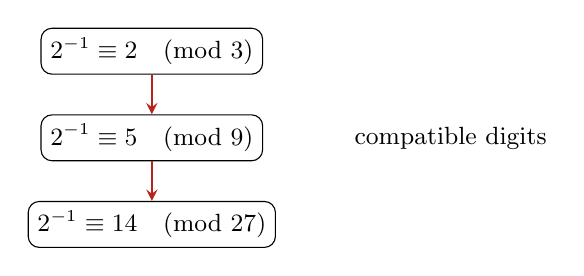
\begin{tikzpicture}[>=stealth,font=\small]
\node[draw,rounded corners] (a) at (0,0) {$2^{-1}\equiv2\pmod3$};
\node[draw,rounded corners] (b) at (0,-1.1) {$2^{-1}\equiv5\pmod9$};
\node[draw,rounded corners] (c) at (0,-2.2) {$2^{-1}\equiv14\pmod{27}$};
\draw[->,BrickRed,thick] (a)--(b);\draw[->,BrickRed,thick] (b)--(c);
\node[right] at (2.45,-1.1) {compatible digits};
\end{tikzpicture}
